\section{Edge Adding Algorithm}


\begin{figure}[htb]
	\begin{algorithmic}
		\renewcommand{\algorithmicrequire}{\textbf{Input:}}
		\renewcommand{\algorithmicensure}{\textbf{Output:}}
		\Require {Integer $k$, k-neighborhood graph $G=(V,E)$}
		\Ensure {Graph $G'=(V,E')$}
		\State {$wList=E$}
		\While {$wList \neq \emptyset$}
			\State {select and remove some $(u,v) \in wList$}
			\State {perform a BFS of length $k$ from $u \in V$}
			\If {BFS reaches $x \in V$ such that $x \not \in N_k(u)$}
				\State {skip}
			\EndIf
			\State {perform a BFS of length $k$ from $v \in V$}
			\If {BFS reaches $x \in V$ such that $x \not \in N_k(v)$}
				\State {skip}
			\EndIf
			\State {add $(u,v)$ to $E'$}
		\EndWhile
		\Return {$G'$}
	\end{algorithmic}
	\caption{Pseudocode for the Edge-Adding Algorithm}

\end{figure}

\begin{figure}[htb]
\centerline{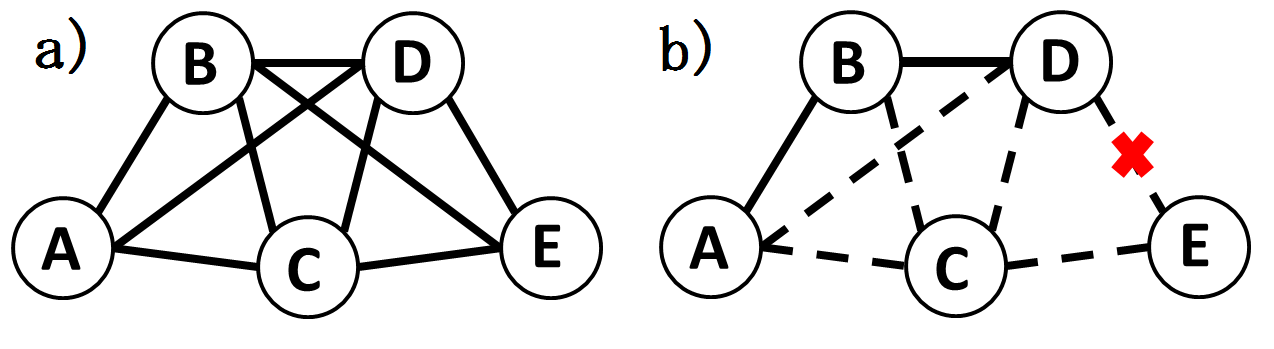
\includegraphics[scale=0.37]{profs_example.png}}
	\caption{An example of the edge-adding algorithm. a) The 3-neighborhood graph for a given input. Each edge in this graph is added to the potential-edge list at the start of the algorithm. b) The solid lines represent edges that will be in the graph the algorithm returns (edge (B,D) was the last edge added). The dotted lines are remaining edges in the potential-edge list. After (B,D) was added, there became a 2-path between A and D. Since E is not adjacent to A in the 3-neighborhood graph, the edge (D,E) was removed from the potential-edge list.}
	\label{fig:edge-adding}
\end{figure}

\begin{figure}[htb]
\centerline{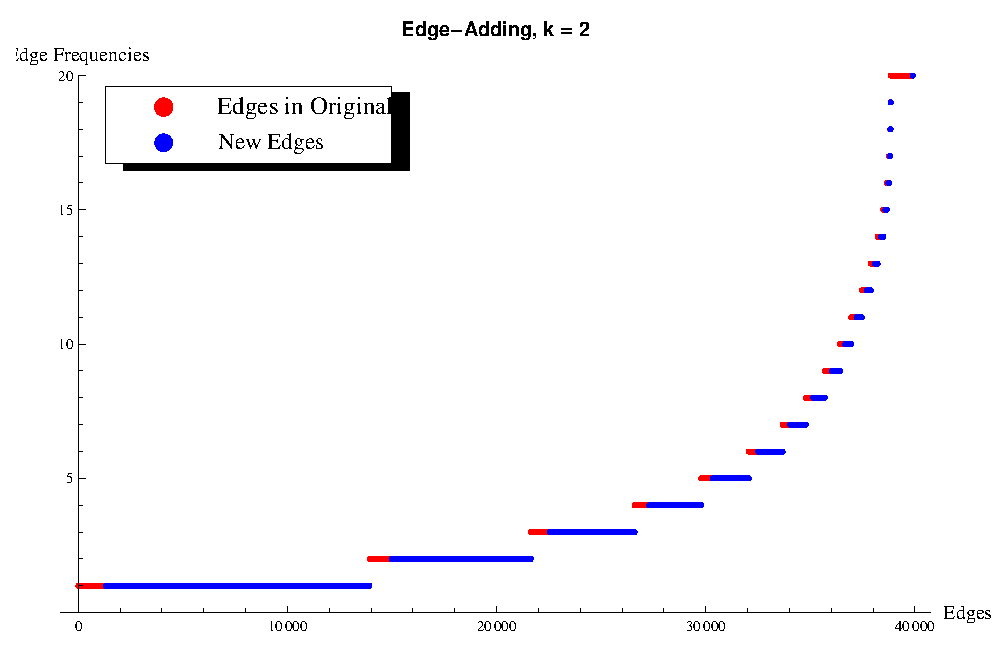
\includegraphics[scale=0.5]{s40_edge_add_k_2.eps}}
	\caption{The results of the edge-adding algorithm when run on the blog data when k=2. }
	\label{fig:edge-adding k=2}
\end{figure}

\begin{figure}[htb]
\centerline{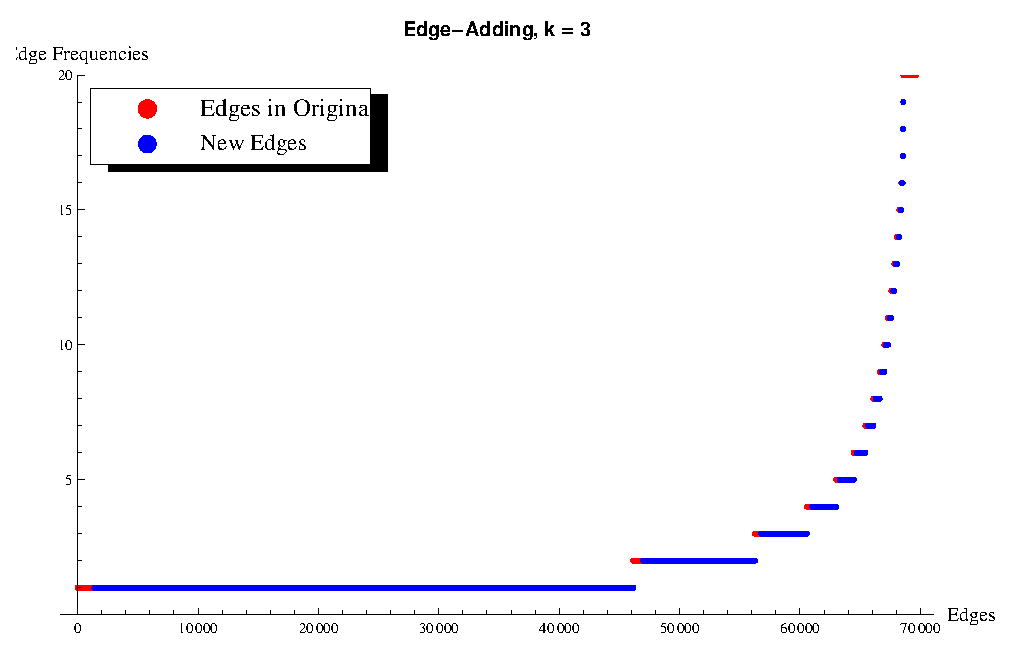
\includegraphics[scale=0.5]{s40_edge_add_k_3.eps}}
	\caption{The results of the edge-adding algorithm when run on the blog data when k=3. }
	\label{fig:edge-adding k=3}
\end{figure}

\begin{figure}[htb]
\centerline{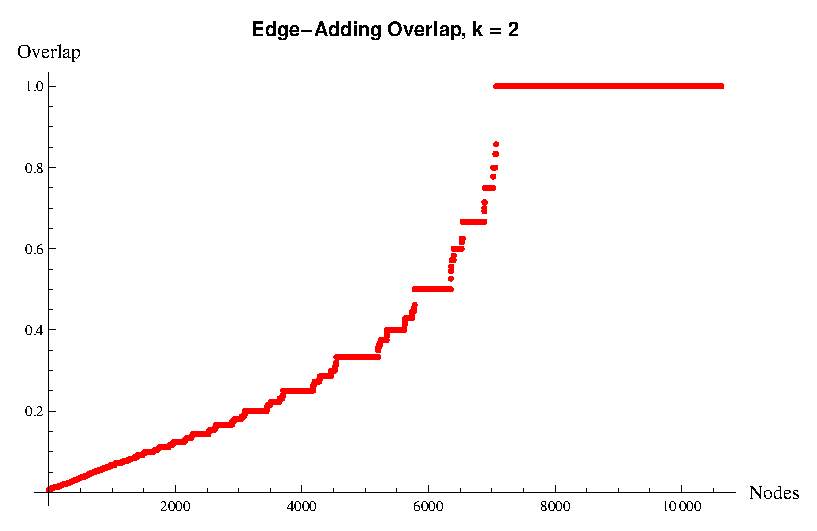
\includegraphics[scale=0.5]{s40_edge_add_k_2_overlap.eps}}
	\caption{The resulting neighborhood overlap between nodes in the initial graph and the graph created by the edge adding algorithm. Overlap between two nodes is measured by the size of the intersection of 2-neighborhoods divided by the size of the union of the 2-neighborhoods. The average overlap is 0.5108 . }
	\label{fig:edge-adding overlap k=2}
\end{figure}

\begin{figure}[htb]
\centerline{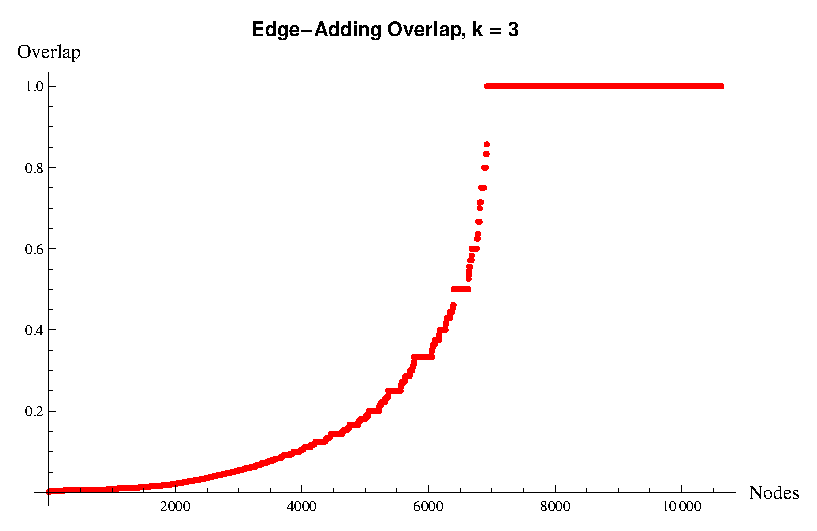
\includegraphics[scale=0.5]{s40_edge_add_k_3_overlap.eps}}
	\caption{The resulting neighborhood overlap between nodes in the initial graph and the graph created by the edge-adding algorithm when k = 3. The average overlap is 0.4432 . }
	\label{fig:edge-adding overlap k=3}
\end{figure}

\indent The edge-adding algorithm, as shown in figure \ref{fig:edge-adding}, is a greedy algorithm which find a graph $G = (V,E)$ that approximately satify a given k-neighborhood graph, $G_k = (V, E')$. The algorithm works to find a graph whose k-neighborhood is at least a subgraph of $G_k$. It begins by adding the edges of $G_k$ into a working list. We know any satisfying graph must be a subgraph of $G_k$, as every edge of a graph must be included in the k-neighborhood of that graph. Therefore, we want to find a subset of our working list that satisfies $G_k$. This algorithm works by iteratively adding edges from the working list to the new graph.  At each iteration, a random edge $(u,v)$ is selected and removed from the working list. A breadth-first search of length $k$ is run from both $u$ and $v$ in the current graph, $G$. If the search (say, from $u$) reaches a node that is not adjacent to $u$ in $G_k$, then we know adding $(u,v)$ to $G$ would invalidate the graph and the edge is discarded. If no such node is found, then $(u,v)$ is added to $G$. This process continues until the working list is empty. This algorithm runs in $O(|E|*d^k)$ time, where $d$ is the maximum node density. As social networking graphs are typically sparse, this algorithm runs in near-linear time. \\

\indent When tested with LinkedIn data, the edge-adding algorithm causes the vast majority of edges in the resulting graph to be new. While it is good that the results do not show the opposite, with most of the edges being those present in the original graph and its mask, this is still not a good result because it can be assumed with very a very high degree of certainty that any given edge in the graph mask is not an edge in the original. It is worth noting that because of the nature of this algorithm, no edges are invalid, which, itself, is a desirable quality. These results do not vary much between between $k$ values of $2$ and $3$. \\
